\documentclass[11pt,a5paper]{article}

\usepackage[T1]{fontenc}
\usepackage[utf8]{inputenc}
\usepackage{lmodern, microtype}
\usepackage[estonian]{babel}
\usepackage{siunitx}
\sisetup{inter-unit-product=\ensuremath{{}\cdot{}}, per-mode=fraction, exponent-product=\cdot, output-decimal-marker={,}}
\usepackage{graphicx}
\usepackage{wrapfig}
\usepackage{adjustbox}
\usepackage{tikz}
\usetikzlibrary{arrows.meta, patterns, patterns.meta}
\usepackage{pgfplots}
\usepackage[european]{circuitikz}
\tikzset{component/.style={draw,thick,circle,fill=white,minimum size=0.75cm,inner sep=0pt}}
\usepackage{amsmath,amssymb}
\usepackage{amsfonts}
\usepackage[hidelinks]{hyperref}
\usepackage{csquotes}
\usepackage{caption}
\usepackage{enumitem}
\topmargin=-3.0cm \textheight=19cm \textwidth=12.9cm
\oddsidemargin=-1.5cm  \evensidemargin=-1.5cm
\setlength{\parindent}{0pt} \setlength{\parskip}{6pt} \sloppy
\sloppy \relpenalty=10000 \binoppenalty=10000
\pagestyle{empty}

\newcommand{\numb}[1]{\vspace{5pt}\textbf{\large #1}}
\newcommand{\nimi}[1]{(\textsl{\small \uppercase{#1}})}
\newcommand{\punktid}[1]{(\emph{#1~p.})}
\newcounter{ylesanne}
\newcommand{\yl}[1]{\addtocounter{ylesanne}{1}\numb{\theylesanne.} \nimi{#1} \newblock{}}
% \newcommand{\autor}[1]{}% Kasuta võistluse ajal
\newcommand{\autor}[1]{\emph{Autor: #1}}% Kasuta kui vaja autorit

\begin{document}

\begin{center}
  \textbf{\Large Eesti koolinoorte 70. füüsikaolümpiaad} \par
  \emph{1. aprill 2023. a. Lõppvoor \\Gümnaasiumi ülesannete lahendused (10.--12. klass)}
\end{center}


\yl{SUJUV AUTOSÕIT}
\punktid{6} \autor{Jaan Kalda}\par
Ei ole sujuv: seismajäämise hetkel muutub hõõrdejõud hetkeliselt nulliks, mis tähendab, et inimesed, kes olid pidurdamise ajal kergelt tahapoole kallutanud, et seista neile jalgade juures mõjuva hõõrdejõu ja toereaktsiooniga paralleelselt, kaotavad tasakaalu ja hakkavad tahapoole kukkuma.

\yl{ELEKTRIKARJUS}
\punktid{6} \autor{Jaan Kalda} \par
Kui elektrikarjuse traat on maapinnast isoleeritud, siis seal voolu pole, pingelangu pole ja järelikult on pinge maa suhtes võrdne elektromotoorjõuga, seega $\mathcal E=\SI {15}{\kV}$. Kui inimene puudutab traati, siis ta sisuliselt lühistab selle, st elektromotoorjõule langeb selle sisetakistus. Elektromotoorjõud $\mathcal E$ sisetakistusega $R$ on ühendatud takistile $r$:
\begin{center}
  \begin{circuitikz}
    \draw (0,0) to[battery1, l=$\mathcal{E}$, invert] (2,0) to[R=$R$] (4,0) -- (4,2) to[R=$r$] (0,2) -- (0,0);
  \end{circuitikz}
\end{center}
Järelikult $R_{\min{}}+r=\mathcal E /I_{\max{}}=\SI{500}{\kohm}$. Näeme, et $r\ll R_{\min{}}$, seega  $R_{\min{}}\approx \mathcal E /I_{\max{}}=\SI{500}{\kohm}$.

\yl{LÄÄTS JA KAKS PEEGLIT}
\punktid{8} \autor{Aigar Vaigu} \par
Tõmbame punktist $A$ väljuva horisontaalse sinise kiire, pärast poolläbilaskvas peeglis peegeldumist on see vertikaalne, läätses koondab selle optilisele peateljele, kus see peegeldub ning jõuab läätseni tagasi. Teiseks kiireks tõmbame lilla kiire punktist $A$ poolläbilaskva peegli keskpunkti, pärast läätse läbimist liigub see edasi otse (kuna läätse fookus on poolläbilaskva peegli keskpunktis) ning lõikub läätse tasandis algse kiirega. Selle punkti näol on tegu $A$ kujutisega. Analoogselt konstrueerime punkti $B$ kujutise läätse tasandis. Objekti $AB$ kujutis läätse tasandis on sama suur kui oli algne kujutis. Tasub märkida, et seda kujutist näeb ülevalt vaadates (kui oleks tegu tavalise peegliga näeks seda ainult poolläbilaskva peegli ja läätse vahel asudes).

Nii algsel objektil kui selle kujutisel läätse tasandis on ka kujutised poolläbilaskvas peeglis nagu oleks neil tavalistes peeglites. Konstrueerime ka need.

Kokku tekib kolm kujutist. Ülemist kujutist näeb altpoolt poolläbilaskvat peeglit vaadates. Parempoolset kujutist näeb vasakult poolt poolläbilaskvat peeglit vaadates. Nagu juba mainitud, siis kujutist läätse tasandis näeme vaadates ülevaltpoolt.

Kuna siin skeemis on poolläbilaskev peegel, siis kujutised on mõnevõrra tumedamad võrreldes tavalise peegliga. Alumine kujutis 2 korda tumedam vaadates seda poolläbilaskva peegli ja läätse vahelt ning 4 korda tumedam vaadates seda läbi poolläbilaskva peegli. Parempoolne ja ülemine kujutis on mõlemad 4 korda tumedamad.
\begin{center}
  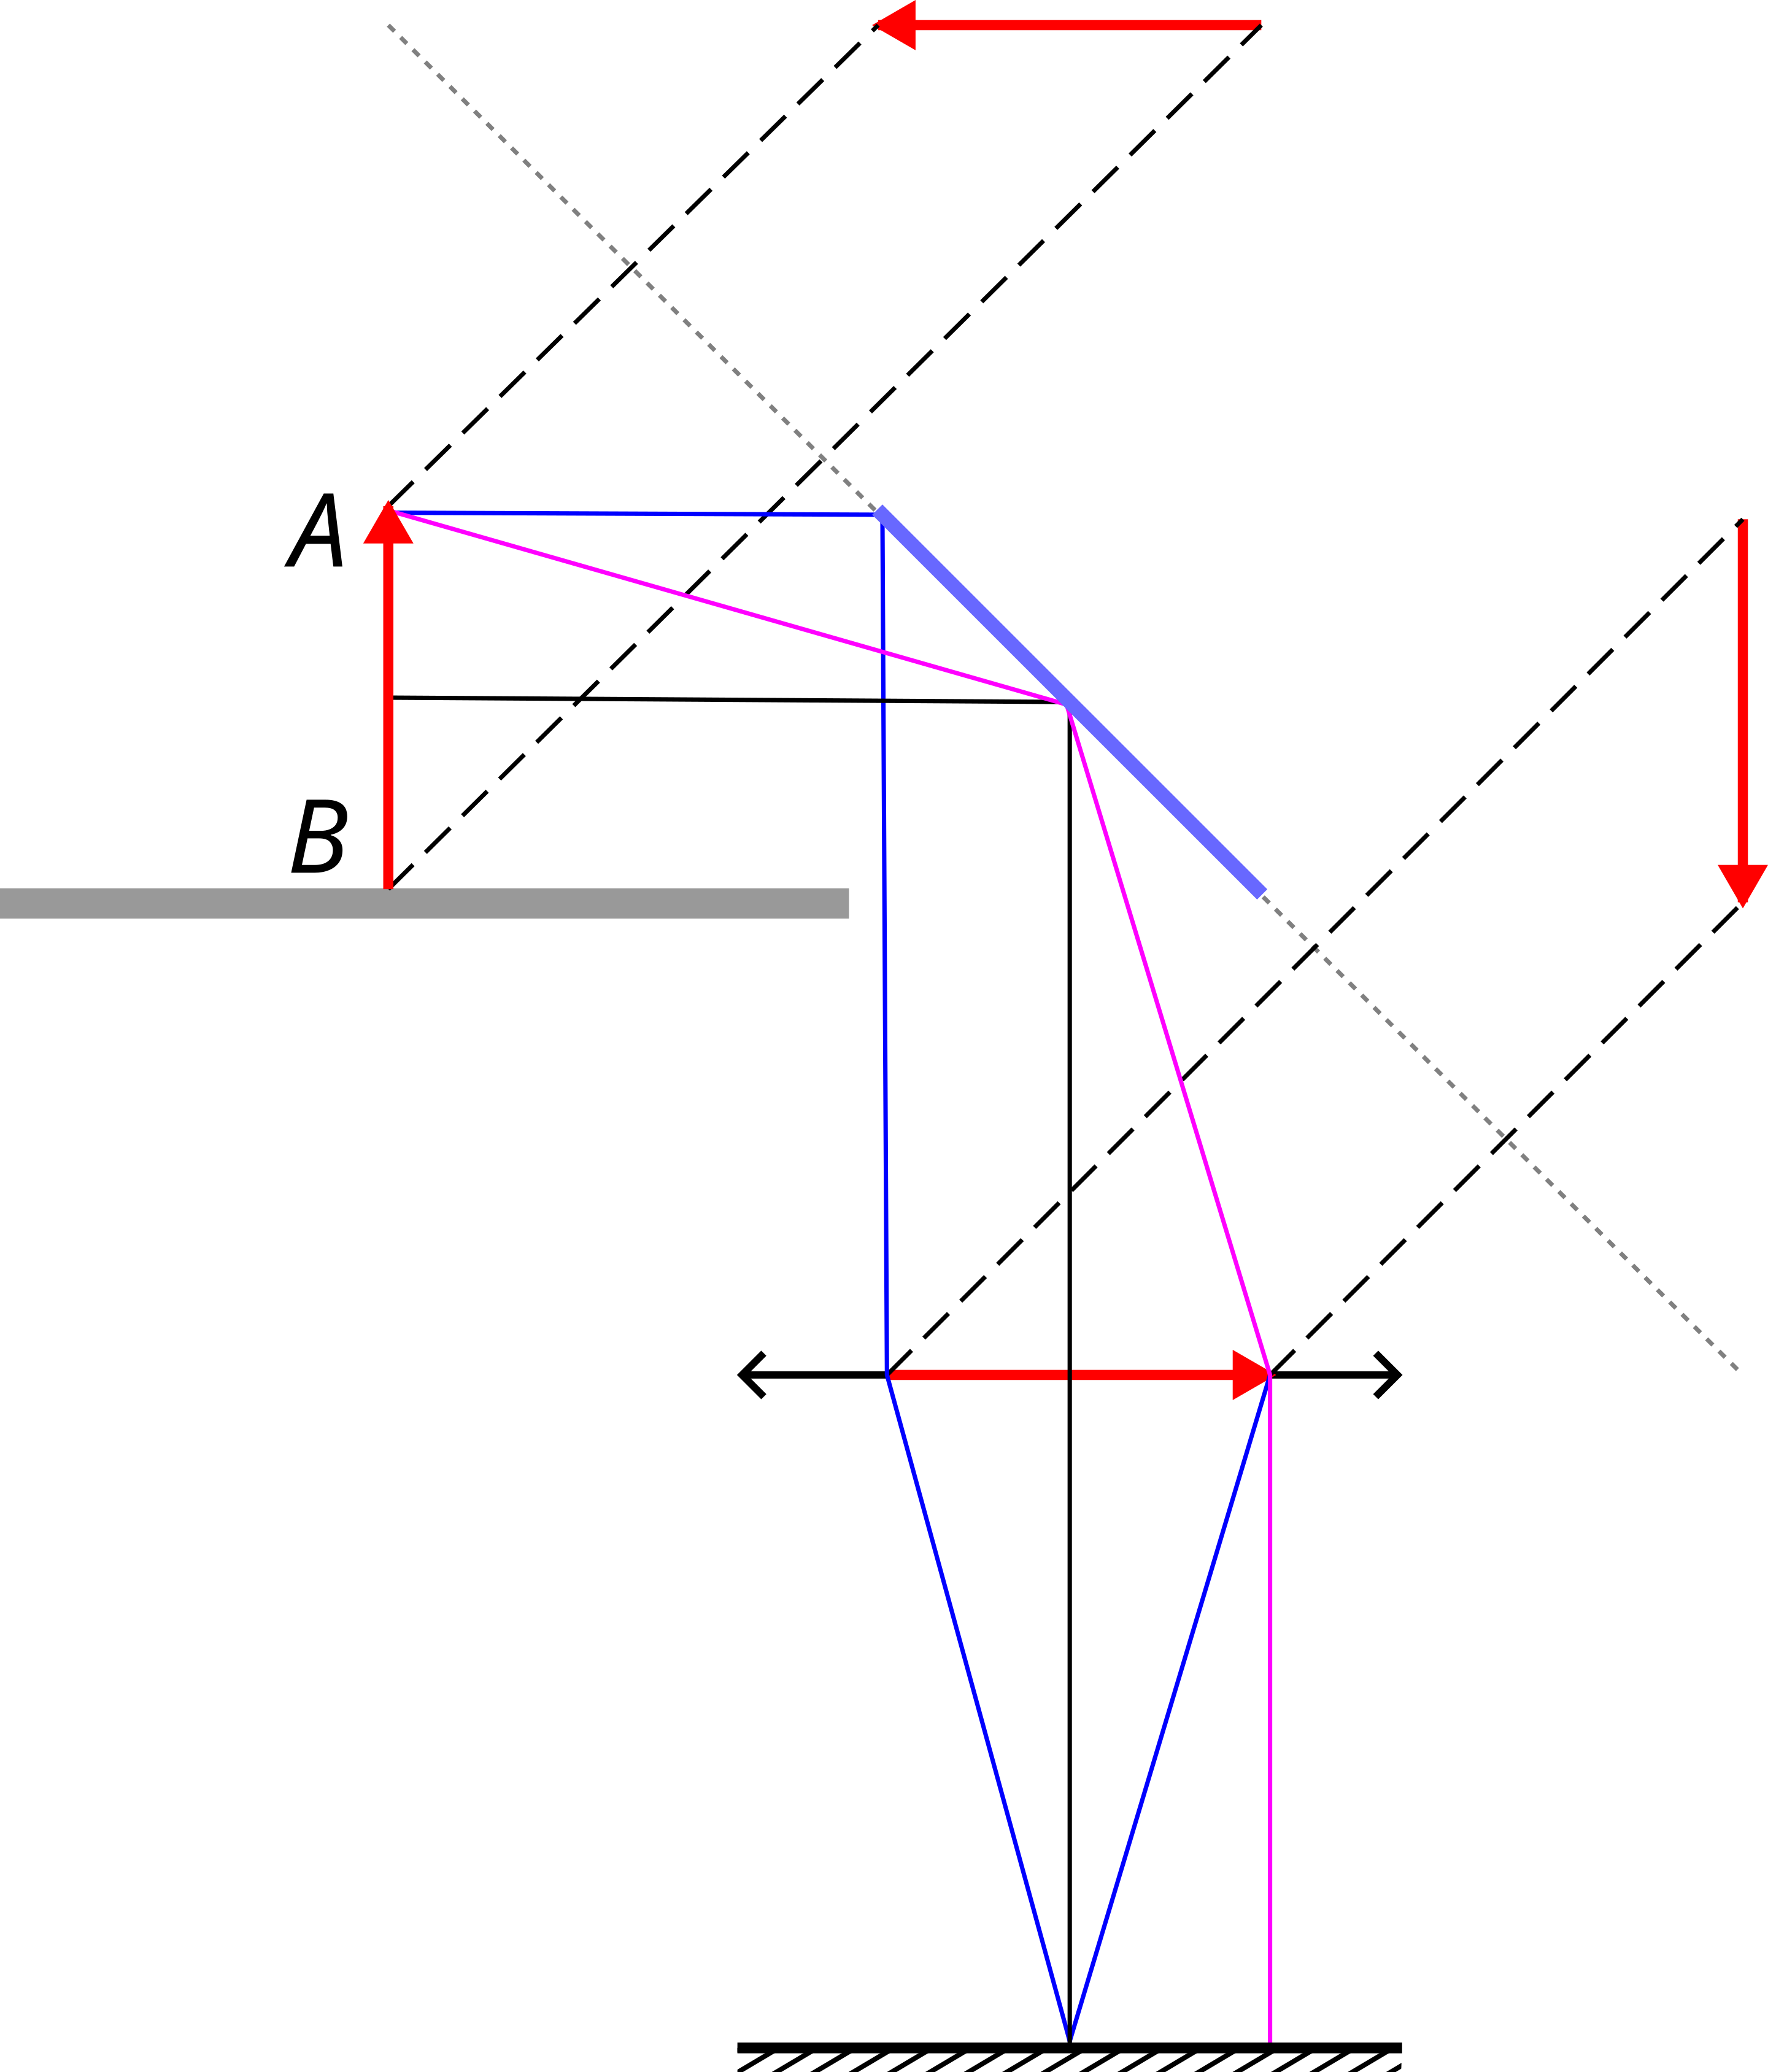
\includegraphics[width=0.86\textwidth]{optika-lah.png}
\end{center}

\yl{Laev}
\punktid{8} \autor{Kaarel Kivisalu} \par
Nurk laeva ja kanali ristsihi vahel on $ \alpha = \arccos (d/l)$. Kanali põhja poolt laevale avaldatav toereaktsioon on $N = (m-\rho lwh k) g$.

Sümmeetri tõttu hakkab laev pöörlema ümber oma keskpunkti. Seega puksiiride efektiivne jõud on risti laeva sihiga. Seega $F \cos \alpha = \mu N/2$. Nendest võrranditest avaldades saame, et
\begin{equation*}
F=\frac{\mu g l}{2d} (m-\rho l w h k).
\end{equation*}

\yl{Sundventilatsioon}
\punktid{8} \autor{Kaur Aare Saar}\par
Loeme juuresolevalt graafikult, et temperatuuril $T_1 = \SI{20}{\celsius}$ on küllastunud aururõhk $p_{k1} = \SI{2340}{\pascal}$ ja temperatuuril $T_2 = \SI{-5}{\celsius}$ on küllastunud aururõhk $p_{k2} = \SI{420}{\pascal}$. Järelikult on toas veeauru osarõhk $p_1 = p_{k1} r_1 = \SI{1170}{\pascal}$ ja õues on veeauru osarõhk $p_2 = p_{k2} r_2 = \SI{336}{\pascal}$.

Olgu õhu ruumala, mis toast kümne tunni jooksul väljub $V$. Sama palju peab tulema ka sisse.
Toast väljuvas õhus oleva veeauru massi $m_1$ saame arvutada ideaalse gaasi valemist:
$$p_1V = \tfrac {m_1}M RT_1.$$
Ja tuppa sisenevas õhus oleva veeauru koguse $m_2$ saame arvutada valemist:
$$p_2V = \tfrac {m_2}M RT_1.$$
Kuna toas on veeauru hulk konstantne, siis järelikult peab õhuniisutis aurustuma sama palju vett kui palju läheb toast välja. Seega saame seose $m = m_1 - m_2$. Järelikult saame avaldada kümne tunniga toast väljuva õhu ruumala:
$$V = \frac{mRT_1}{M(p_1-p_2)} = \SI{160}{\meter\cubed}.$$
Õhu vahetumise kiiruseks seega saame $\SI{16}{\meter\cubed\per\hour}$.

\newpage
\yl{Nõel vees}
\punktid{10} \autor{Marten Rannut}\par
Ülesandes kirjeldatud olukord on ligikaudu näidatud joonisel. Veepind pisut kõverdub ning seeläbi pindpinevusjõuga tasakaalustab nõela raskusjõu. Pindpinevusjõud mõjub veepinna sihis kontaktpunktides (see ei pruugi olla tangentsiaalne nõela pinnaga nagu on joonisel näidatud, kuid ülesande lahendust see ei mõjuta). Kummalegi poolele nõelast mõjub jõud $\sigma \ell$. Kui pindpinevusjõu vektorid on horisontaali suhtes nurga $\alpha$ all, siis saame jõudude tasakaalust \(mg = 2 \sigma \ell \sin \alpha\). Kuna veepind on sama nurga all kui jõuvektorid, siis otsitav nurk on
\[
\alpha = \arcsin{\frac{mg}{2\sigma \ell}} \approx \SI{34}{\degree}.
\]
\begin{center}
  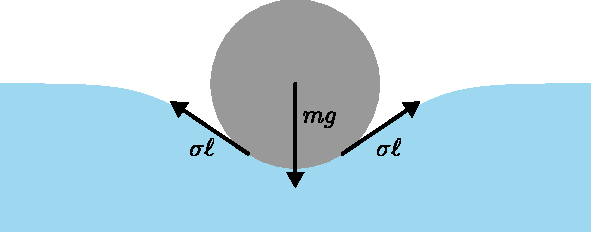
\includegraphics[width=9cm]{noel-lah.pdf}
\end{center}

\yl{TEHISKAASLANE}
\punktid{10} \autor{Eero Vaher}\par
Paneme tähele, et orbiidi kaugeimas punktis peab tehiskaaslase kiirusvektori projektsioon tehiskaaslast planeedi keskmega ühendavale lõigule olema $0$. Kui kiirusvektori projektsioon oleks positiivne, liiguks tehiskaaslane planeedist eemale ning tehiskaaslane oleks järgmisel ajahetkel planeedist kaugemal. Kui kiirusvektori projektsioon oleks negatiivne, oleks tehiskaaslane planeedile lähemale liikumas ning tehiskaaslane olnuks eelmisel ajahetkel planeedist kaugemal.

Ringorbiidil oleva keha jaoks on kesktõmbejõuks gravitatsioonijõud ehk $\frac{mv^2}{r}=\frac{GMm}{r^2}$, kus $G$ on gravitatsioonikonstant, $M$ planeedi ning $m$ tehiskaaslase mass. Järelikult $GM=v^2r$.

Vaatleme esmalt juhtu, kus tehiskaaslasele antaks kiirendus selle liikumissuunas. Vahetult pärast kiirenduse saamist oleks tehiskaaslase kiirus $u_1=v+\Delta v=\frac{31}{24}v$. Selle koguenergia oleks $E_1=\frac{mu_1^2}{2}-\frac{GMm}{r}$ ning selle impulsimoment $L_1=mru_1$. Olgu tehiskaaslase kiirus orbiidi kaugeimas punktis $w_1$. Impulsimomendi jäävuse põhjal $L_1=mR_1w_1$ ehk $w_1=\frac{r}{R_1}u_1$ ning energia jäävuse põhjal $E_1=\frac{mw_1^2}{2}-\frac{GMm}{R_1}$ ehk $\frac{u_1^2}{2}-v^2=\frac{u_1^2r^2}{2R_1^2}-\frac{v^2r}{R_1}$. Selle saame teisendada kujule $\left(\frac{u_1^2}{2}-v^2\right)R_1^2+v^2rR_1-\frac{u_1^2r^2}{2}=0$. Selle võrrandi lahendid on $R_1=\frac{-v^2r\pm\sqrt{v^4r^2-2v^2u_1^2r^2+u_1^4r^2}}{u_1^2-2v^2}=\frac{-v^2r\pm\sqrt{\left(1-2\left(\frac{31}{24}\right)^2+\left(\frac{31}{24}\right)^4\right)v^4r^2}}{\left(\frac{961}{576}-2\right)v^2}=\frac{1\mp\left(\frac{961}{576}-1\right)}{\frac{191}{576}}r$. Suurim kaugus oleks järelikult $R_1=\frac{961}{191}r=\SI{277729}{km}$.

Kui kiirendus oleks suunatud planeedist eemale, oleks tehiskaaslase kiirus vahetult pärast kiirenduse saamist $u_2=\sqrt{v^2+\Delta v^2}=\frac{25}{24}v$. Selle koguenergia oleks $E_2=\frac{mu_2^2}{2}-\frac{GMm}{r}$ ning impulsimoment $L_2=mrv$. Olgu tehiskaaslase kiirus orbiidi kaugeimas punktis seekord $w_2$. Impulsimomendi jäävuse põhjal $L_2=mR_2w_2$ ehk $w_2=\frac{r}{R_2}v$ ning energia jäävuse põhjal $\frac{u_2^2}{2}-v^2=\frac{v^2r^2}{2R_2^2}-\frac{v^2r}{R_2}$ ehk $\left(\frac{u_2^2}{2}-v^2\right)R_2^2+v^2rR_2-\frac{v^2r^2}{2}=0$, mille lahendid on $R_2=\frac{-v^2r\pm\sqrt{v^4r^2-2v^4r^2+v^2u_2^2r^2}}{u_2^2-2v^2}=\frac{-v^2r\pm\sqrt{\left(\frac{625}{576}-1\right)v^4r^2}}{\left(\frac{625}{576}-2\right)v^2}=\frac{1\mp\frac{7}{24}}{\frac{527}{576}}r$. Suurim kaugus oleks järelikult $R_2=\frac{24}{17}r=\SI{77928}{km}$.

\yl{Kuulitõuge}
\punktid{10} \autor{Valter Kiisk}\par

Kuna kuul on raske ja selle kiirus on väike, siis õhutakistuse panus on praegusel juhul tühine. Optimaalse viskenurga erinevus \ang{45}-st on seega tingitud peamiselt sellest, et alg- ja lõpp-punkt ei paikne samal kõrgusel. Ülesande sirgjooneliseks lahendamiseks tuleks avaldada kuuli lennukauguse $s$ sõltuvus viskenurgast $\alpha$ ja määrata selle maksimum. See tee viib väga tülikate avaldisteni. Ülesande saab siiski lahendada alternatiivsel viisil.

Arvestades, et kuuli algkõrgus maapinnast on $h_0$, avaldame kõigepealt lõpp-punkti kõrguse (mis on võrdne nulliga):
\[
0=h_0+v_{0y}t-\frac{1}{2}gt^2,
\]
kus $v_{0y}=v_0\sin\alpha$ ja kuuli lennuaeg
\[
t=\frac{s}{v_{0x}}=\frac{s}{v_0\cos\alpha}.
\]
Seega
\[
0=h_0+s\tan\alpha-\frac{gs^2}{2v_0^2}\cdot\frac{1}{\cos^2\alpha}.
\]
Peale trigonomeetrilise seose $1/\cos^2\alpha=1+\tan^2\alpha$ kasutamist saame ruutvõrrandi $\tan\alpha$ suhtes. Selle füüsikaliselt mõistlik lahend on
\[
\tan\alpha=\frac{v_0^2}{gs}+\frac{1}{gs}\sqrt{v_0^4+2gh_0v_0^2-g^2s^2}.
\]
Seega kui $h_0$ ja $v_0$ on fikseeritud, siis saadud avaldis annab sellise sobiva viskenurga, mille korral kuuli lennukaugus saab olema $s$. Kuid meid huvitab selline viskenurk, mille korral $s$ on maksimaalne ($=s_\text{m}$). Järelikult, kui viimases avaldises $s$ võtta suurem maksimaalsest võimalikust väärtusest, peab saadav $\tan\alpha$ väärtus väljuma füüsikaliselt võimalikest piiridest, st reaalarvude vallast. Piirjuht saavutatakse siis, kui ruutjuurealune avaldis (diskriminant) saab võrdseks nulliga:
\[
v_0^4+2gh_0v_0^2-g^2s_\text{m}^2=0.
\]
See on tingimus kuuli algkiiruse määramiseks. Tegemist on ruutvõrrandiga $v_0^2$ suhtes, mille lahendiks on
\[
v_0=\sqrt{g\sqrt{s_\text{m}^2+h_0^2}-gh_0}\approx \SI{13.3}{m/s}.
\]
Viimaks otsitava algnurga tangens avaldub
\[
\tan\alpha=\frac{v_0^2}{gs_\text{m}}=\frac{\sqrt{h_0^2+s_\text{m}^2}-h_0}{s_\text{m}},
\]
millest $\alpha\approx\ang{42}$.

\yl{Staatiline elekter}
\punktid{12} \autor{Jaan Kalda}\par
Metalli pinnal paiknevad laengud ümber nii, et metalli sees oleks elektrivälja tugevus null. See tähendab, et kile alla koguneb kilega võrdne ja vastasmärgiline pindlaeng pindtihedusega $-\sigma=-Q/S$, kus $Q$ on kilel olev kogulaeng.

Kile tekitab metalli pinnal elektrivälja tugevusega $E=\sigma/2\varepsilon_0$; selle saab tuletada kas Gaussi teoreemist või plaatkondensaatori mahtuvuse valemi $C=\varepsilon_0 S/d$ arvestades, et plaatide vahelisse välja panustavad mõlemad plaadid võrdselt, st kumbki tekitab välja tugevusega $E=U/2d$, kus $U$ on kondensaatori pinge ja $d$ on plaatide vahekaugus. Paneme tähele, et kile materjali elektrist läbitavust $\varepsilon$ me ei pea mängu tooma, sest vaatleme elektrivälja vahetult metalli kohal, plaadi ja kile vahelises mikroskoopilises õhupilus. Metalli pinnale indutseeritud laengule $-Q$ mõjub jõud $F_C=QE=2\varepsilon_0E^2S$. Selle kompenseerib toereaktsioon $N=F/\mu$, tänu millele jõuame võrrandini
\[
  F=2\mu\varepsilon_0E^2S\Rightarrow E=\sqrt{F/2\mu\varepsilon_0S}.
\]
Kui viia kile kaugusele $h$, siis laengute pindtihedused kilel ja metallil ei muutu, ja seetõttu ei muutu ka väljatugevus kille ja plaadi vahel, st plaadi ja kile vaheline pinge on leitav kui $U'=2Eh$; tegur 2 tuleneb siin sellest, et praegu vajame kile ja plaadi vahel olevat summaarset välja tugevust $2E$, mitte ühe plaadi tekitatud väljatugevust $E$. Niisiis
\[
  U'=h\sqrt{2F/\mu\varepsilon_0S}=\SI{42}{\kV}.
\]

\yl{Uppuv pall}
\punktid{12} \autor{Jaan Kalda}\par
Teeme joonise valguskiire käigu kohta silmast palli ülemise ja alumise servani. Need on veepinnal murduvad jooned, mis on peaaegu paralleelsed, kui vaadelda pallilähedast piirkonda, sest palli mõõtmed on hulga väiksemad kaugusest (mis on ilmselt suurem kõrgusest $H=\SI 2\m$). Alumiste sirgete osade vahekaugus $a$ on võrdne palli diameetriga, ülemiste sirgete osade vahekaugus $b$ vastab palli näivale kõrgusele. Ülaltvaates palli vasakusse ja paremasse serva tõmmatud sirged näiliselt ei murdu, seega pallin näiv laius on võrdne palli tegeliku laiusega. Seega on palli näiv lapikus $k=a/b=3$. Kui tähistada murdjoone ülemise osa kaldenurga veepinna suhtes $\beta$-ga ja alumise osa kaldenurga $\alpha$-ga, siis saame eelpooltoodud tingimusest johtuvalt seosed $a=d\sin\alpha$ ja $b=d\sin\beta$, kus $d$ tähistab murdjoonte murdepunktide kaugust. Seega saame võrrandi $\sin\alpha=k\sin\beta$ ning murdumisseadusest  $\cos\alpha=\cos\beta/n$. Võttes need avaldised ruutu ja liites vasakud ning paremad pooled saame $1-n^{-2}=(k^2-n^{-2})\sin^2\beta$, millest $\sin\beta=\sqrt{7/135}$. Silma kaugus pallist $L=H/\sin\beta=H\sqrt{135/7}\approx\SI{8.8}\m$.

\end{document}